The interplanetary transfer time has a big impact on the design. The transfer time determines for instance the mass for food of the astronauts, the amount of radiation they need to endure, how much they need to exercise and more. Keeping the transfer time short will minimise these problems. However it will also increase the $\Delta\gls{sym:V}$-budget needed for the launcher. 

\begin{figure}[h]
	\centering
	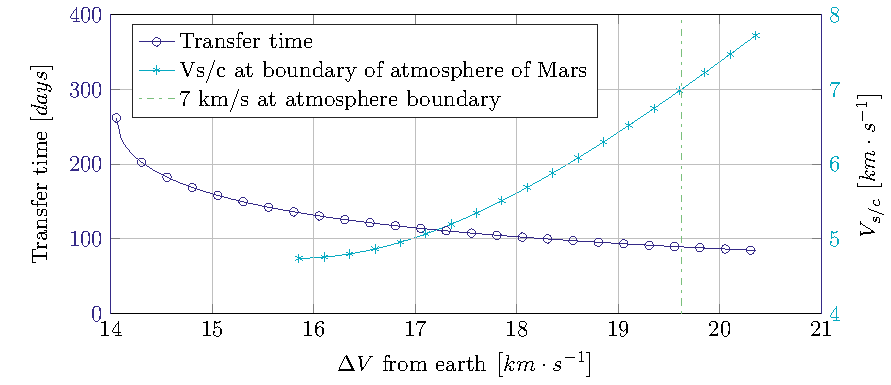
\includegraphics[width=0.95\textwidth]{Figure/Inter_transfer/transfer_time.pdf}
	\caption[Interplanetary transfer time and entry velocity versus $\Delta\gls{sym:V}$]{Interplanetary transfer time (left) and entry velocity (right) versus $\Delta\gls{sym:V}$}
	\label{fig:inter_time}
\end{figure}

The most efficient travel with respect to $\Delta\gls{sym:V}$ consists of a Hohmann transfer orbit. This would take approximately 262 days. This time is the longest of all orbits with a direct transfer. One of the mission requirements is the entry velocity of 7 $\left[km \cdot s^{-1}\right]$, this velocity is mainly determined by the $\Delta \gls{sym:V}$ budget and therefore determined by the transfer time. In figure \ref{fig:inter_time} this relation is visualised. As can be seen to arrive with the required velocity a $\Delta \gls{sym:V}$ of $19.62$ $\left[km \cdot s^{-1}\right]$ is required, which corresponds to a transfer time of 89.3 $\left[days\right]$. The corresponding orbit is shown in figure \ref{fig:inter_orbit}.

\begin{figure}[h]
	\centering
	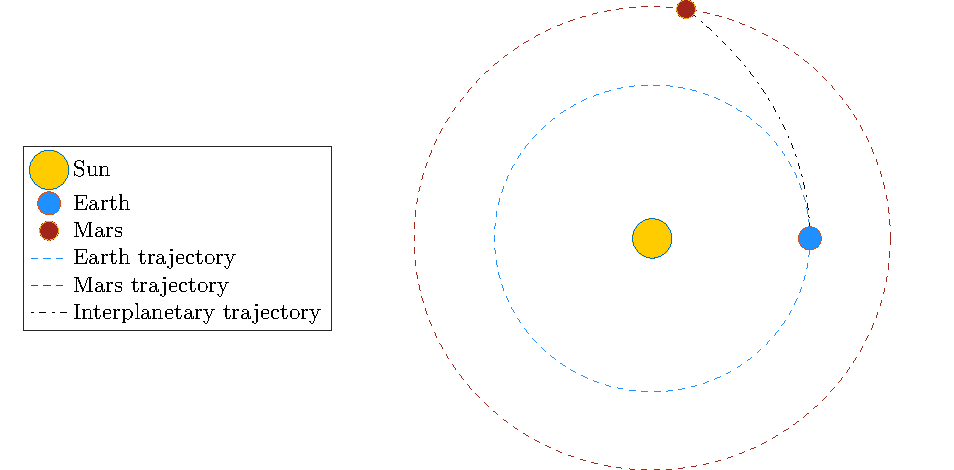
\includegraphics[width=0.95\textwidth]{Figure/Inter_transfer/orbits.pdf}
	\caption{Visualisation of the interplanetary transfer orbit}
	\label{fig:inter_orbit}
\end{figure}
